% !TEX root = ../main.tex
\chapter{IoT Brain} \label{ch:framework}

This chapter is going to give some informations about the design choice taken while implementing the approaches in \textbf{\autoref{ch:model}} and \textbf{\autoref{ch:diagnosis}}.
Implementation efforts were aimed at providing a further degree of scalability to the approach and leveraging cloud based technologies as well as reducing the technical difficulties that usually arise while fiddling with complex tools like Semantic Web ontologies that are, in turn, too expressive for the scope of this project.

\section{Fully integrated BMS}
Previous chapters defined a possible approach, developed by IBM Research, for diagnosing smart buildings. It has been shown that such a method works as expected. However such instruments needs to be integrated in a broader panorama of services that should be present in a Smart Building, instead of being perceived as standalone, monolithic applications. Defining the term Smart Building is a challenging task and various organizations adopt their own definition.
The US Government Services Administration (GSA):
\begin{quote}
Technology alone won’t do it. The GSA realises that the smartest part of smart buildings is people and wants to engage them. Providing feedback and information through a dashboard is a good start. With smart technology, we can learn anything we want about a building and optimise its performance. But real performance means happier, more productive tenants. And that requires insights into the hears and minds of the people inside. What a dashboard can really do is enable better decisions, inspire participation, spread knowledge and best practices, communicate at a human scale and propagate new norms in how we use our buildings.
\end{quote}
while IBM states:
\begin{quote}
Smart buildings are well managed, integrated physical and digital infrastructures that provide optimal occupancy services in a reliable, cost effective, and sustainable manner. Smarter buildings help their owners, operators and facility managers improve asset reliability and performance that in turn, reduces energy use, optimizes how space is used and minimizes the environmental impact of their buildings.
\end{quote}
many others provide their own definitions that, however,  do not change that much, if not in the form. What emerges is that a smart building has to be an integrated set of applications that works and communicate in order to enable the building to perceive the context it is in, being aware of its status and its occupants. Another key concept it is its ability to react, and adapt, autonomously to changes in the environment, possibly predicting meaningful  events and optimizing its behaviour in order to optimize occupants comfort and energy consumption.
IoT devices provide the context for a Smart Building. Commercial buildings are constantly monitored by IoT smart sensors and meters (see \autoref{fig:iot_growth}) that provide a huge amount of data that needs to be stored and processed, aggregated and enriched with external data sources to extract useful information on the state of the building.
\begin{figure}
  \centering
  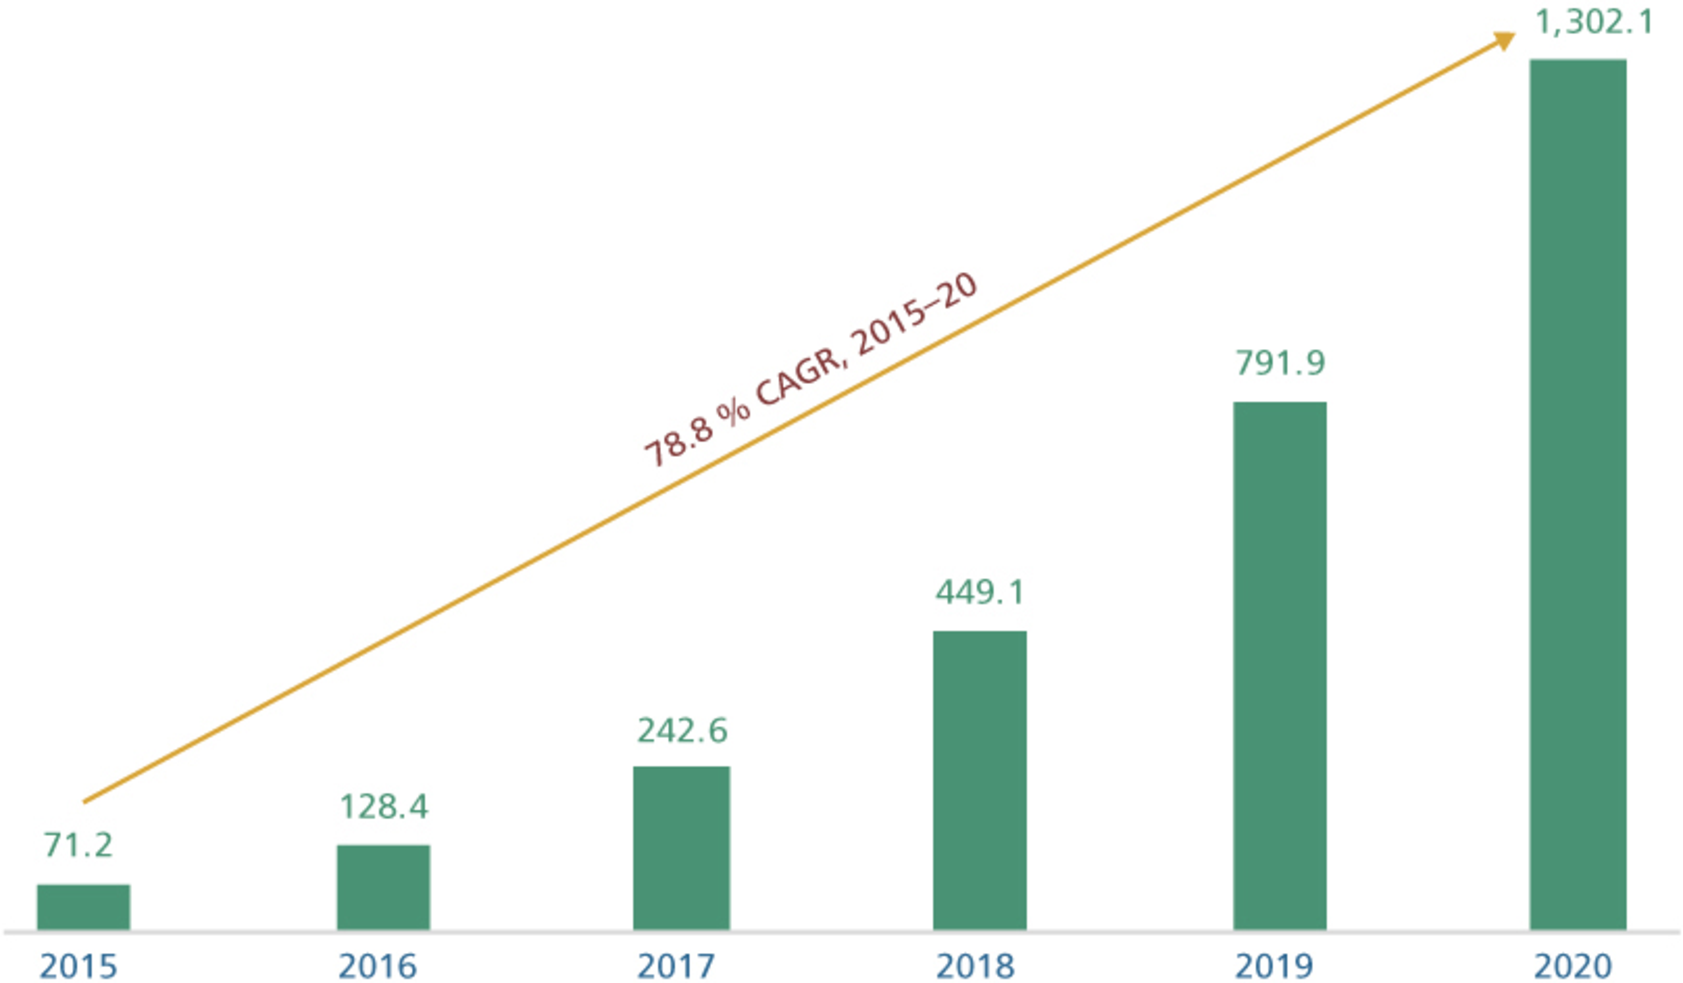
\includegraphics[width=.8\textwidth]{iot_growth.pdf}
  \caption{Potential growth in worldwide IoT sensor deployements for Commercial Real Estate, [millions]}
  \label{fig:iot_growth}
  \source{Chart created and analysis performed by the Deloitte Center for Financial Services based on Gartner research: ``Forecast: Internet of Things, endpoints and associated services, worldwide, 2015'', Gartner Inc., October 29, 2015. Graphic: Deloitte University Press | DUPress.com}
\end{figure}
Analytics provide the means that the building use to interpret the context and react in a correct way (diagnosis, user comfort models, energy consumption predictions). An example can help to better understand the concept of fully integrated and smart BMS. Let a fault occour at a Fan Coil Unit (FCU) in a room. A Smart Building should be able to detect it, diagnose it, alert the manager, eventually issue a repair request to the maintenance service with a description of the fault. Then, upon arrival of the maintenance worker, the building should be able to guide said worker through the building itself towards the location of the fault with a human-like conversational interface.
Through the example it is higlighted the strong integrated nature of a Smart Building Management and Automation System.

\section{Requirements} \label{sec:requirements}
In a Smart Building context it is important to understand what are the main goals that are to be achieved by the deployment of such a system. What emerged from this thesis work is that a Smart Building IT infrastructure needs to be build upon a scalable framework that provides a platform for easy and fast analytics deployement. There's a need of a middleware that provide every top level application with a common ground that abstract the physical sensors so that the whole system is integrated and top layer components are able to exchange informations. This middleware is born from the Semantic Web concept of ontology (see \autoref{ch:semantic_web}) and of semantic reasoning. What is different here is that the scope is note the same. Semantic Web technologies have their focus on massive amount of diverse data that comes from different sources and their goal is somewhat to unify them and give them a meaning that is universally accepted. That is a hard goal to achieve for a single simple ontology. Therefore highly complex solutions like the Ontology Web Language (OWL)\cite{owl_reccomendation} have been developed. In that context standardization and rigid formality in their representation. In the context of Smart Buildings the focus is shifted and requirements become more lax.
Building's data are sensible and are not supposed to be exchanged outside of the scope of a single organization (a company, a university, etc.), additionally, since the goal of this framework is to manage a building, the concepts involved are little in numbers and simpler in structure than those involved in the Semantic Web. \textcite{brick_schema} showed how a little number of concepts and relationships (see \autoref{fig:brick_schema}) is required for capturing the complexity of a building. Orthogonal to this, another simple ontology SSNO and its extension (see \autoref{subsec:ssn}), developed by IBM Research, suffice for capturing the complexity of physical interaction between buildings assets, as seen in \autoref{fig:extended_ssno}.
Moreover, opposed to the Semantic Web context, it can't be forget that a part of the integrated system is comprised of human actors who work and live in the buildings and form a big part of the context of the building itself. It is important to identify and focus on the potential users of such a system. Those users are both those who benefit from the deployed analytics and those who are going to develop those analytics, still it is not required from them to have a strong computer science background of any sort; even developers in this case can be just domain expert (eg. physicists, civil engineers etc.) that for example needs to update, or change, the physical model rules or the model of the architecture. The system should aim at providing those users the most straightforward default way to interact with the system, trough high-level languages and possibily human language interfaces (see \autoref{sec:conversational_interface}) yet it should still allows for low level interaction where needed. To sum it up, the system that is the end goal of the project needs:
\begin{itemize}
  \item easy development tools
  \item high level scripting languages
  \item semantic capabilities to enable integration
  \item scalable back-end
\end{itemize}

\section{Knowledge Inference Technology for IoT}
Knowledge Inference Technology for IoT (KITT) is a layered framework that provide an API to model, manage and reason on the semantic knowledge of IoT Systems. It has been developed by IBM Research and expanded with further capabilities as the core of this thesis. It is designed to meet the requirements outlined in the previous section and to provide a service for integrated deployment of analytics in IoT contexts.
KITT adopt a layered approach as seen in \autoref{fig:kitt}.
\begin{figure}
  \centering
  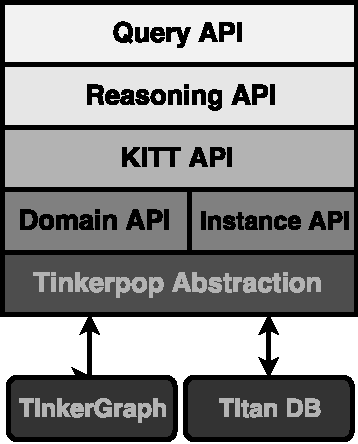
\includegraphics{kitt.pdf}
  \caption{KITT internal structure}
  \label{fig:kitt}
\end{figure}
Each of these layers implements different functionalities that will be detailed just below

\subsection{TinkerPop abstraction layer}
This layer is strictly related to the low level implementation of the graph on the physical store. What is important to note is the choice of representation of the underlying RDF graph that is the base of the semantic approach. Altough many RDF stores and semantic databases are available, the choice made fell towards a graph Data Base (DB) implementation of said RDF graph. The main reason is to be searched in the scalability needs of the project and the scope of it. What has been developed is an integrated semantic framework for Smart Buildings and not a multipurpose layered semantic engine.
\paragraph{GraphDB vs. RDFStore}
It is important to note that the word semantic doesn't necessarly mean RDF. When talking about semantic it is intended a way to give a meaning to otherwise unmeaningful data so that more complex operations can be performed, thanks to the abstraction that such additional knowledge provide. It has been said in \autoref{subsec:rdf} that RDF is a way to store triples, and that those triples represent a graph. Ontologies, then, are still triples that makes use of some well known concepts and relationships (e.g Class and subClassOf) to give a meaning to RDF triples. It follows that RDF data, both ground truth and ontologies, can be safely stored in a graphDB. There are also some advantages in using a graph representation. For instance, graph DB implements the so called Labeled Property Graph (LPG) whose main advantage is that of storing vertexes and labels that can have an internal structure. In practice, this allows for the chance of storing additional data, whose semantic description is not essential, without complicating the ontology. It is possible, for example, to store information about geographical coordinates of an equipment directly in the node, without having to model such data in the ontology (see \autoref{subsec:kitt_api}). This way applications can also append (e.g through JSON string) other application-dependant data at runtime, keeping the model small in size.
\paragraph{Apache TinkerPop}
The TinkerPop abstraction layer has been developed in order to abstract the underline storing engine and provide vendor indipendance. This layer provide a series of methods that can be used by upper layers to directly operate on the graph without worrying about the underline technology. Changing the graphDB engine just requires the right implementation of the abstraction layer without further modification of the upper layers. Apache TinkerPop itself is an open source, vendor-agnostic, graph computing framework distributed under the commercial friendly Apache2 license.

\subsection{Domain API and Instance API}
These layers both work upon the TinkerPop Abstraction layer as they are the main component involved while building the model of a building. The domain API acts when defining the taxonomy of a domain. For example, whenever it is needed to express that a new concept exists, like a Room is a subClassOf a Location, that is Domain API duty. The Instance API is, instead, in charge of the creation of new facts, that are the specific knowledge about a system. This API is the one responsible, for example, of the creation of new instances, such that Room0408 is a instance of the concept Room. In \autoref{fig:dom_inst_api} it is detailed which API an instance and a concept are going through when they are created in the graph.
\begin{figure}
  \centering
  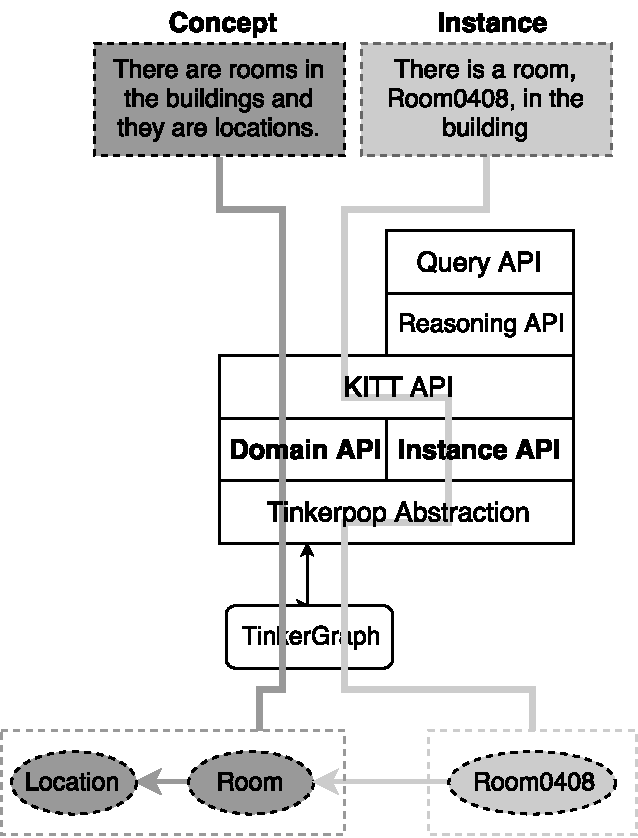
\includegraphics[width=.4\textwidth]{conc_inst_api.pdf}
  \caption{Usage of the Domain and Instance API}
  \label{fig:dom_inst_api}
\end{figure}

\subsection{KITT API}\label{subsec:kitt_api}
KITT API is the middle ground between lower layers and upper layers. At this point of the stack everything is abstract enough so that the main focus shift towards the user of the system, be it human or an application. KITT API provide high level endpoints that allow for interactions with the lower level domain and instance endopoints through high level text base format (JSON, KITT scripting).

\paragraph{KITT scripting}
KITT scripting language is a way for the end user to inject in the system a whole model in a straightforward way. A end user should be able to load a whole model without worrying about implementation details or technical aspects of reasoning and ontology modelling. This lead to the development of a simplified scripting language for ontology creation, that is simple yet expressive enough for implementing the needed relationships of Brick (\autoref{subsec:brick}) and SSN (\autoref{subsec:ssn}) ontologies. It is based on the following assumptions:
\begin{itemize}
  \item Domain concepts and relationships are structured in a taxonomy and so are disjointed
  \item Relationships can be established between concepts or between instances
  \item Relationships between concepts and instances are only the basic ones connecting an instance to its parent concept
  \item Instances have to be instantiated from the defined model.
\end{itemize}
Thanks to these assumptions the scripting language can define a full model in a human readable text format. Under these assumptions the model is powerful enough to create a digital twin of the building. A KITT script is divided into three main parts
\begin{itemize}
  \item Concepts definition
  \item Model instantiation
  \item Ruleset definition.
\end{itemize}
In the concept level definition a series of concepts, that is the vocabulary of the model, are defined as shown in \autoref{lst:kitt_concept_def}
\begin{lstlisting}[label={lst:kitt_concept_def}, caption={KITT script for domain definition}, breaklines=true]
[Init]
[Dimensions]
Point
Location
Equipment
Property
[InstanceReferenceTypes]
hasLocation = in
hasPoint
isFedBy
hasProperty
[Concepts]
Location
  Room
Equipment
  HVAC
    AHU
Point
  Sensor
    Flow_Sensor
      Supply_Air_Flow_Sensor
    Temperature_Sensor
Property
  Temperature
\end{lstlisting}
the script start with the definition of the main dimensions of the ontology. In \autoref{lst:kitt_concept_def} the definition of Point, Location, Equipment and Measurement suggests that the ontology used is going to be Brick. The \verb|[InstancereferenceTypes]| section introduce which possible relationships are going to be instantiated later, shorthands can be defined so that defining instances, in the appropriate section of the script, becomes easier. The \verb|[Concept]| tag start the part of the script where the taxonomy of the ontology is defined. The tabulation at the start of each line has a semantic meaning and defines the hierarchy of the concepts; An indent means that the following concepts are sub-concepts of the upper one, while concepts on the same line represent disjointed classes. In it is represented the scripting module that correspond to the declaration of the ground truth of the knowledge base, that in the case of a smart building that means defining the architecture, the spatial relationships between locations and the various equipment and points distributed in the buildings.
\begin{lstlisting}[label={lst:kitt_instance_definition}, caption={Definition of instances}, breaklines=true]
[Instances]
Room1708 a Room ``the room''
  TS1708 a Temperature_Sensor hasPoint Room1708 X{"type": "Point", "coordinates": [32.76473, 35.01616] }X {oBMS:"ts\1708\."}
AHU1 a AHU isFedBy Room
  SAF_U1 a Supply_Air_Flow_Sensor hasPoint AHU1
...
\end{lstlisting}
the instantiation is done through the keyword \verb|a|, that specify the concept an isntance belongs to. While creating the instance the KITT interpreter looks for \verb|X{...}X| GeoJSON coordinates and \verb|{"key":"value",...}| dictionaries and store them in the underline graph node. This allow for a powerful annotation feature enabled by underline property graph structure. For example coordinates can be used by a navigational interface that guides a user in the building.
The next section in a KITT script is the \verb|[Reasoning]| one, whose goal is to define and execute the ruleset that infer the physics model of the building. \autoref{lst:kitt_reasoning_definition} defines the syntax in the script, while the syntax and the meaning of the rules is described in \autoref{subsec:reasoning_api}.
\begin{lstlisting}[label={lst:kitt_reasoning_definition}, caption={Definition of reasoning ruleset}, breaklines=true]
[Reasoning]
Room(x)->Temperature(y)&hasProperty(x,y)
...
\end{lstlisting}
When fed to the KITT API the KITT script goes through a parser that build the model and execute the reasoning. At the time of model creation, the parser itself automatically compute subsumption relationships for the instance such that every instance is directly bound to its parent class and to other ancestor classes.


\subsection{Reasoning API}\label{subsec:reasoning_api}
Whenever reasoning is involved, it is intended as the capability of inferring new knowledge about the system given previous asserted facts and an ontology. The main duty of the reasoning engine in this project is that of applying knowledge about general physics to the given model. The second one is it's capacity of answering complex query that the KITT API level can't natively handle. Therefore KITT reasoning language describe an union of production rules languages like SWRL\cite{swrl_reccomendation} and query languages like SPARQL\cite{sparql_reccomendation}. On top of that ad-hoc functions have been added so that such language could be the most straightforward for the operations involved in this project.
\paragraph{KITT reasoning language}
The reasoning language developed borrowed syntax from classic rule languages like SWRL, yet it needed to expose methods useful to explicit complex query and path traversal. A KITT rule is expressed as a form of entailment \[body\implies head\] where $body$ and $head$ are both expressed in conjunctive form, so that a rule assume the form \[A_1\land\ldots\land A_n\implies B_1\land\ldots\land B_m\] where $A_i$ and $B_j$ are either statements about, or relationships between, facts (see \autoref{eq:rule_facts_only}).
\begin{equation}
\label{eq:rule_facts_only}
Room0408\land Temp0408\implies hasProperty(Room0408, Temp0408)
\end{equation}
That means that wether the condition in the body holds, the condition on the left must hold too. This characteristic, typical of production rules, is used to entail new knowledge according to domain expertise. When coupled with the concept of variable, rules becomes a powerful tool to enforce knowledge on a knowledge base. Thanks to variable, rules can be wrote refering to concepts, that in turn are set of instances; this allows for the encoding of domain expertise into procedural rules. For example, a human expert would not say something as in \ref{eq:rule_facts_multiple}
\begin{equation}
\label{eq:rule_facts_multiple}
\begin{gathered}
Room0408\implies hasProperty(Room0408, Temp0408)\land Temp0408\\
Room709\implies hasProperty(Room709, Temp709)\land Temp709\\
\dots
\end{gathered}
\end{equation}
but would instead say ``Every room has an internal temperature''; from this sentence it emerge that there exist a concept of room, a concept of internal temperature and that this concepts are related. Introducing variables it becomes a rule as in \autoref{eq:simple_prod_rule}
\begin{equation}
\label{eq:simple_prod_rule}
Room(x)\implies Temperature(y)\land hasProperty(x,y)
\end{equation}
where $x$ and $y$ are variables that can be bound to any given fact in the instance model; if the variables appears on the right-hand side of the rule and can't be bound to any given fact in the knowledge base, they are created so that the entailment is satisfied.
The second fundamental function of the reasoner is its capability of answring complex queries. Complex queries are questions whose answers are not imeediately retrievable from the knowledge base through simple relationships. Complex queries are, in contrast with production rules, usually focused on retrieving information about well known facts instead of general knowledge thus requiring for a way of mixing in the same rule both named facts and variables. A good example of this sounds like ``Which are the temperature sensors of the rooms fed by AHU1''; translating it like explained just above
\begin{equation}
AHU(a)\land Room(r)\land isFedBy(r, a)\land TempSensor(t)\land hasPoint(r,t)
\end{equation}
lead to an erroneous interpretation of the query as this would fetch ``every temperature sensor of the rooms that are fed by either one of all the AHUs''
\begin{equation}
AHU(AHU1)\land Room(r)\land isFedBy(r, AHU1)\land TempSensor(t)\land hasPoint(r,t)
\end{equation}
is the right way to go and it has been implemented in the reasoner as \begin{equation}
AHU(a, \# AHU1)\land Room(r)\land isFedBy(r, a)\land TempSensor(t)\land hasPoint(r,t)
\end{equation}
where $AHU(a, \# AHU1)$ binds the variable $a$ to the named individual $AHU1$.
A less traditional ways to use this kind of rules is for the evaluation of property chains. Property chains, in the context of physical modelling and diagnosis represents important knowledge (see \autoref{sec:potential_causes}) and the ability to traverse them is essential for reasoning in such environments. An ad-hoc operator has been introduced so that such traversal are possible
\begin{verbatim}
 _CHAIN({R(dir),R(dir),...}, start, end)[condition]
\end{verbatim}
where \verb|R| is a relationship in the ontology, \verb|dir| $\in$ \verb|[^,v]| tells wether the relationship to chase is an incoming or out-coming one and when are combined as in \verb|{R(dir)...}| they specify a pattern to match; \verb|start| identify a known variable in the head of a rule and so is \verb|end|, respectively identifying the first and last instances of the chain, \verb|condition| is either a number specifying the maximum number of pattern matching to perform before stopping, a condition the \verb|end| variable needs to uphold in order to stop the recursion or both. Such function is visible in \autoref{fig:property_chain_rule}. In the case that a cycle is identified during the traversal it is natively dealt with using standard cycles detection algorithms.
\begin{figure}
  \centering
  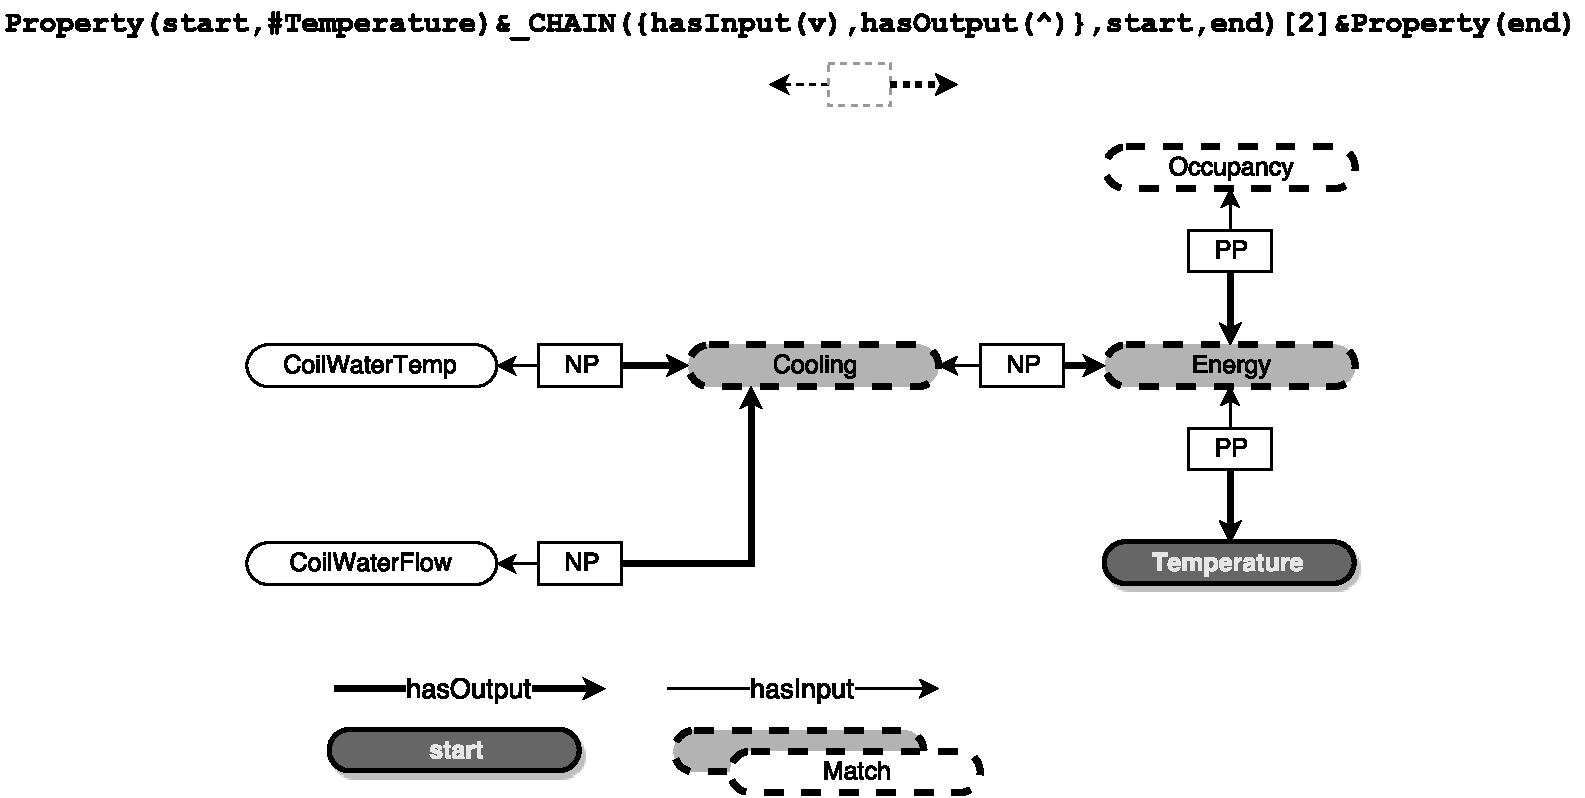
\includegraphics[width=.8\textwidth]{property_chain_rule.pdf}
  \caption{Property chain in a rule}
  \label{fig:property_chain_rule}
\end{figure}
\paragraph{Reasoner known limitations}
It is important to note that enabling the reasoner to perform update/modification of a knowledge base is bound to end up in the domain of undecidable languages. This is easily demonstrated by a counterexample like
\begin{equation}
  A(x)\implies A(y)
\end{equation}
or again
\begin{equation}
  \begin{gathered}
    A(q)\implies B(r) \\
    B(s)\implies A(t)
  \end{gathered}
\end{equation}
and whatever ruleset such that there's some kind of cicles involved in the resolutions of such rules that would start to be fired endlessly and never comes to an halt. Such problem is well known in literature and needs to be evaluated on a case-by-case basis. It boils down to balancing whether is better to achieve high expressivness or remain in the domain of decidability. In this project, given the requirements in \autoref{sec:requirements} has been deemed more appropriate the first than the latter and this follows from the main purpose of the reasoner, that is to fill incomplete knowledge. Another limitation of the current reasoner is represented by the method used for executing the ruleset, that is the most naive possible and is a simple execution based on declaration order.

\section{Towards conversations}\label{sec:conversational_interface}
The whole project has been built upon the concept of semantic layer. This semantic layer is the common ground that allows applications to communicate. The actors involved in a Smart Building, as stated in \autoref{sec:requirements}, are both applications and human users, that are consumers of informations that the building produce on par with other applications. It then makes sense to exploit this semantic common ground to allows end user to interact with the buildings in the most natural way, that is through speech, thus tearing down the barrier between humans and cyber physical systems (CPS). This allows for improved integration of the human resource in the Smart Building system, improving productivity and comfort of the occupants. \autoref{fig:conversational_advantages} shows how the possibility of communicating through a conversational interface allows for increased mobility and it cuts on learning curves, diminishing user frustration when faced with the problem of learning new things.
\begin{figure}
  \centering
  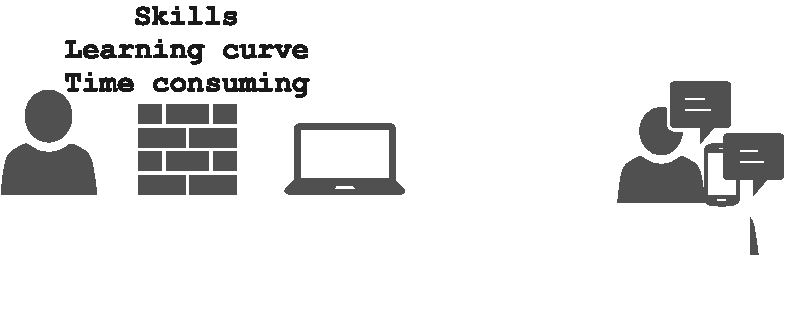
\includegraphics{conv_adv.pdf}
  \caption{Advantages of conversational interface}
  \label{fig:conversational_advantages}
\end{figure}
The main idea behind the approach is that natural language carries a meaning and if the domain context is well defined and agreed upon, it is possible to extract from a natural language sentence enough informations so that it is possible to start a dialogue. In the case of smart buildings the domain context is defined by the vocabularies of Brick and SSN. As soon as a user wants to interact with the system, it can state its question through natural language; the statement is parsed looking for:
\begin{itemize}
  \item concepts, that are the subjects, predicates and objects (thus can be searched for in the ontology)
  \item intents, that specify some kind of processing executed on the subjects and objects.
\end{itemize}
This high-level idea has been implemented thanks to the IBM Watson Conversation services and led to the development of a succesful demo application. More details will be presented in Chapter 5.
% This interaction has been developed, as a proof of concept, using IBM Watson Conversation Service that provide a developing framework for the development of Personal Digital Assistants (PDA). The digital assistant, available through a web service on a mobile friendly web page, was able to distinguish and answer two kind of questions involving complex queries. The demo PDA can distinguish between two kind of intents
%\begin{itemize}
%  \item ``What is'', the simplest intent that has been given the meaning return the object of the query
%  \item ``How many'' that involved the counting of a query result objects.
%\end{itemize}
%The concepts involved where locations, assets and events, so that
